\subsection{Candidate Models}
Given the baseline performance of the pretrained VGG16 with Places image preprocessing, a set of candidate models are proposed with the aim of 1) improving accuracy and 2) reducing dimensionality of feature vectors allowing for faster computation of similarity matrix.
The results from \autoref{sec:baselinemodels} would suggest, that out-of-the-box performance for autoencoder architectures may perform better in producing well-defined encodings from VGG16's fc\_1-layer using Places image preprocessing. 

\paragraph{Pretrained Model with Denoising Autoencoder} \\~
Several configurations of pretrained models with denoising autoencoders have been attempted throughout experimentation. 
Generally autoencoders in this setting tend to perform better when the first encoder layer is of similar dimensions to the input feature vector. 
Broader bottlenecks also tend to retain more information after training, see \nameref{appendix: C}

It would appear, that models trained on input preprocessed with Simple or ImageNet preprocessing schemes achieve significantly lower accuracies compared to models trained on Places preprocessed data. 
Furthermore, models with Places pretrained weights perform better across the board, all else equal. 


\paragraph{Pretrained Model with Deep Autoencoder} \\~
Initial experiments with deep autoencoders show no significant boosts to performance in using either ResNet50 or VGG16 compared to the denoising counterparts. 
Deep autoencoders can be said to perform on-par with narrower denoising autoencoders. They do however take longer to converge. 
Results from experiments on Deep Autoencoders are presented in Appendix C.

\paragraph{Pretrained Model with Deep Denoising Autoencoder} \\~
Adding noise to deep autoencoders yields slightly worse results in terms of accuracy compared to any of the previous approaches. 

\begin{table}[H]
  \centering
  \resizebox{\textwidth}{!}{%
  \begin{tabular}{@{}llllllll@{}}
  \toprule
  Pretrained   & Architecture     & Noise & Preprocessing & Test Acc.      & Val. Acc.      & Top-5 Test Acc. & Top-5 Val. Acc. \\ \midrule
  VGG16 & 4096, 2048, 1028 & 0.3   & Places        & \textbf{0.764} & \textbf{0.753} & \textbf{0.919}  & \textbf{0.913}  \\
  VGG16 & 4096, 2048, 1028 & 0.5   & Places        & 0.74           & 0.735          & 0.908           & 0.904          
  \end{tabular}%
  }
  \caption{Performance of DAEs}
\end{table}
More results for DDAEs with pretrained layer alternation can be found in Appendix C, \autoref{fig:godeeper}.

\paragraph{Pretrained Model with Autoencoder} \newline
In later experiments it was shown, that the best candidate model was obtained by not using more sophisticated autoencoder architectures, but that shallow autoencoders without noise outperformed every other model and the baseline.
\begin{table}[H]
  \centering
  \resizebox{\textwidth}{!}{%
  \begin{tabular}{@{}lllllll@{}}
  \toprule
  Pretrained   & Architecture  & Test Acc.               & Val. Acc.               & Top-5 Test Acc.         & Top-5 Val. Acc.         \\ \midrule
  VGG16(fc\_1) & 4096, 2048           & \textbf{0.782 (+ .013)} & 0.773 (+ .013)          & 0.937 (+ .008)          & 0.944 (+ .017)          \\
  VGG16(fc\_1) & 4096, 3072          & 0.778 (+ .009)          & 0.765 (+ .005)          & 0.943 (+ .014)          & 0.940 (+ .013)          \\
  VGG16(fc\_1) & 4096, 512           & 0.771 (+ .002)          & \textbf{0.783 (+ .023)} & \textbf{0.945 (+ .016)} & \textbf{0.951 (+ .024)} \\
  VGG16(fc\_1) & 4096, 128          & 0.775 (+ .006)           & 0.774 (+ .014)          & 0.936 (+ .007)          & 0.944 (+ .017)          \\ \bottomrule
  \end{tabular}%
  }
  \caption{Experimentation with AEs (Places preprocessing), parentheses indicate improvement over baseline}
  \label{fig:finaltable}
\end{table}

In \nameref{sec:trainae}, it is suggested that adding regularization in the bottleneck layer improves performance for autoencoders. 
Naïve trials, adding L1-regularization with $\lambda = 0.001$ to the bottleneck layer were attempted - but all experiments yielded lower accuracies across all metrics.
Thus, regularization has not been used in the proposed models - and the results on regularization have been omitted from this paper for the sake of brevity.

\subsection{Model Evaluation}
In the above section, minute improvements over the best baseline model were observed. 
This section produces a more in-depth, side-by-side comparison of the best-performing candidate model, in terms of test/val accuracy.
The shallow VGG16-AE-512 with Places image preprocessing from \autoref{fig:finaltable} achieves the best overall results among all candidate models. 
Furthermore, it outperforms the baseline on every metric.

\begin{figure}[H]
  \centering
    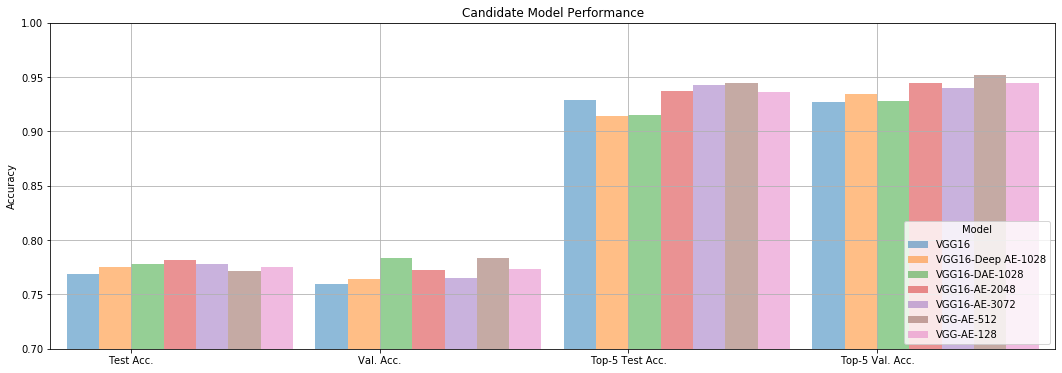
\includegraphics[width=\textwidth]{pictures/plots/final_cand_perf}
    \caption{Candidate Model Accuracies v. Baseline}
    \label{fig:candidates}
\end{figure}

\subsubsection{Model Predictions}
The best AE model, appears to have grasped very detailed image features in a feature vector smaller by a factor of 8 compared to the VGG16(fc\_1) forward passes.
In \autoref{fig:aepredictions_full} predictions on the test set are shown using the encodings from the VGG16-AE-512 model:
\begin{figure}[H]
  \centering
  \begin{subfigure}[b]{0.47\textwidth}
    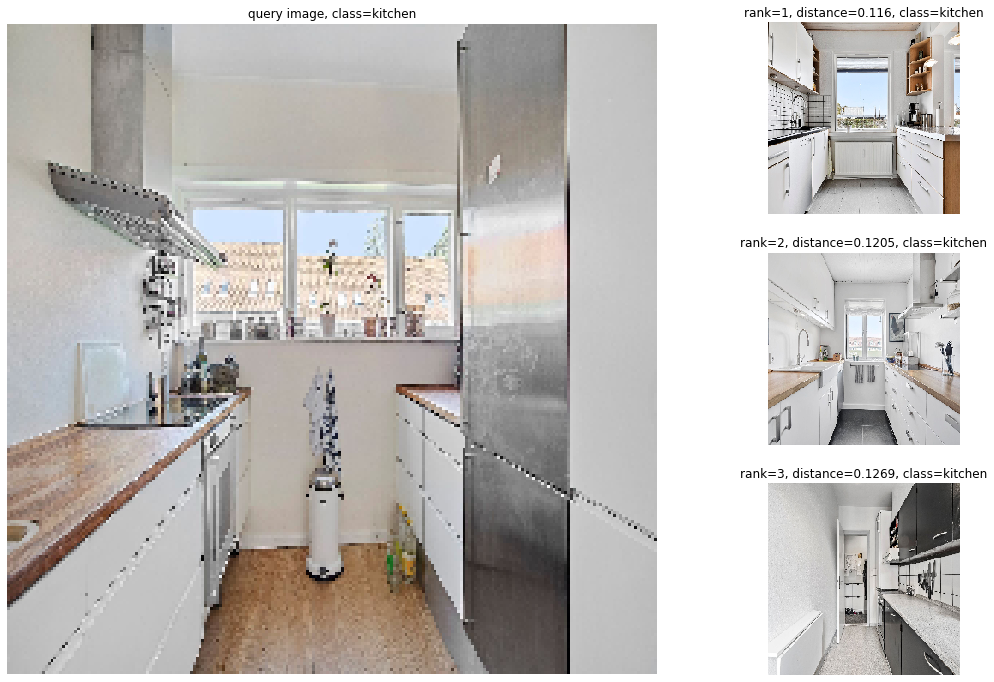
\includegraphics[width=\textwidth]{pictures/plots/kitchen_4_test}
  \end{subfigure}
  %
  \begin{subfigure}[b]{0.47\textwidth}
    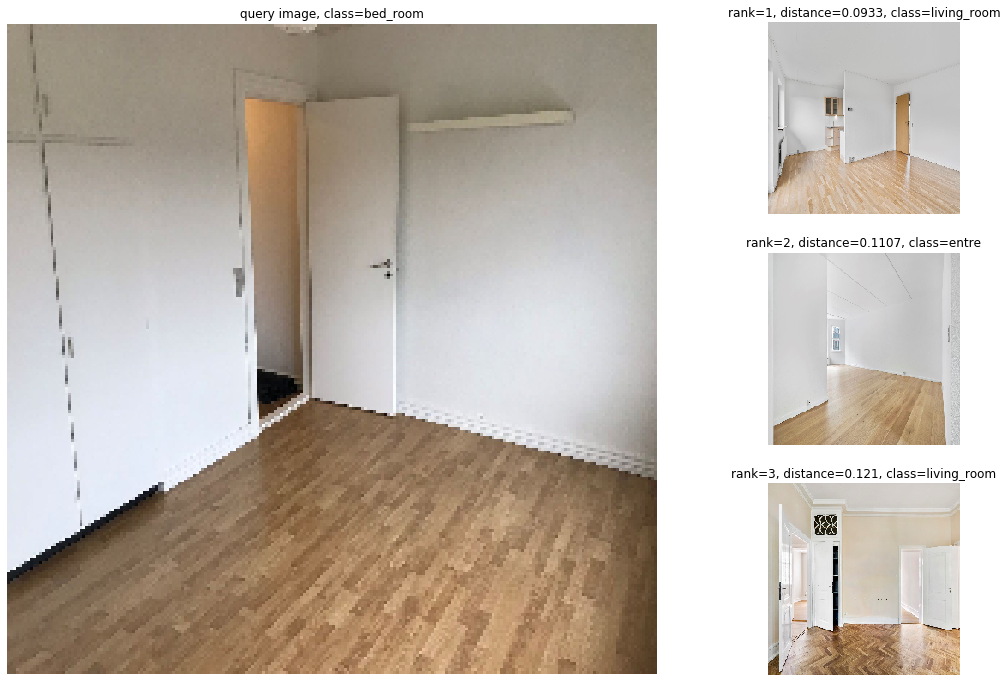
\includegraphics[width=\textwidth]{pictures/plots/bed_room_237_test}
  \end{subfigure}
  \caption{VGG16-AE-512 Predictions }
  \label{fig:aepredictions_full}
\end{figure}
More predictions by VGG16 and VGG16-AE-512 on more classes can be found in \nameref{appendix: D}.
\newline
\newline
In order to get and understanding of the models it is useful to map the feature vectors of a model into a 2-dimensional space using \texttt{t-SNE}\autocite{Chu2017}\autocite{HintonScience2006}. 
As suggested in \autocite{wattenberg2016how}, several combinations of hyper parameters were tested on train, test, and validation data; see \nameref{appendix: E}.
For all configurations, the DAE produces a lower KL-divergence, indicating that VGG16-AE-512 has learned a representation better at separating images that would otherwise be clustered together.

\begin{figure}[H]
    \centering
    \begin{subfigure}[b]{0.47\textwidth}
      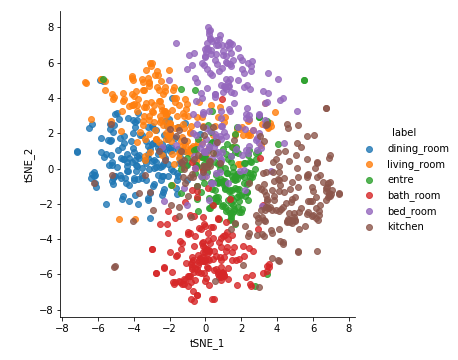
\includegraphics[width=\textwidth]{pictures/plots/tsne_vgg16}
      \caption{t-SNE: VGG16, p=50}
      \label{fig:tsne1}
    \end{subfigure}
    %
    \begin{subfigure}[b]{0.47\textwidth}
      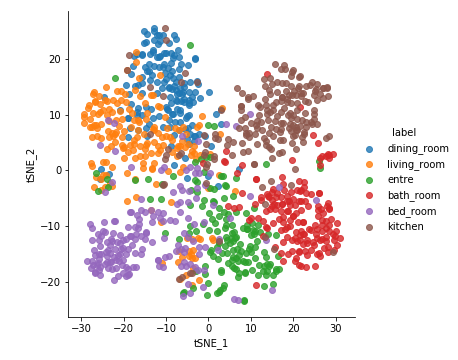
\includegraphics[width=\textwidth]{pictures/plots/tsne_vgg16_dae}
      \caption{t-SNE: VGG16-AE-512,  p=50}
      \label{fig:tsne2}
    \end{subfigure}
    \caption{t-SNE Comparison of feature vectors}
    \label{teesnee}
\end{figure}
